\chapter{Tree Refinement}
\label{chap:tree}
% 0.5 Seiten

	With the existing capabilities of \ac{GCG} presented in the previous chapter, we continue with the main contributions of this thesis:
	
	\begin{itemize}
		\item A new module which is integrated into the detection framework of \ac{GCG} for reverse engineering semantic groupings of the original formulation. This can be seen as a generalization of the approach presented in \cite{}
		\item Additional auxiliary classifiers which implement constraint and variable classification based on information not currently used including examples of \textit{when} they are crucial detecting semantics.
	\end{itemize}

	This chapter is divided into three main section:
	
	\begin{enumerate}
		\item A short summary about the available information we have access to.
		\item What the motivation and goals are why and how we aim to process this information.
		\item The concrete algorithm and its most integral parts.
	\end{enumerate}
	
	Some concrete details about the implementation itself are not subject of the following sections, but are discussed in Chapter \ref{chap:impl}.

	\clearpage

	\section{Information}
	% 1 Seite
	
	\begin{figure}[ht!]
		\centering
		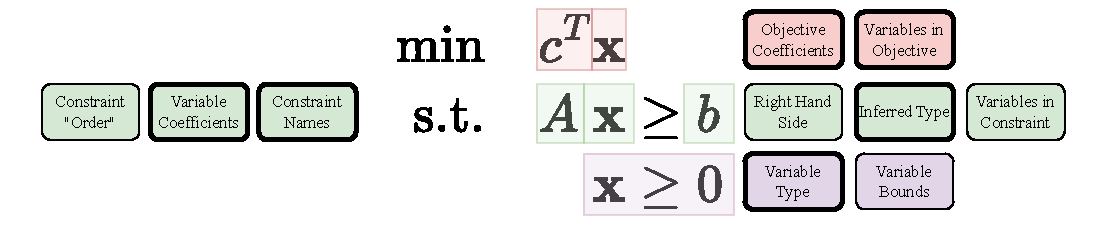
\includegraphics[scale=0.8]{Bilder/DrawIO/model_information}
		\caption{All parts of a model that contain useful information for semantic grouping of constraints and variables. Elements with a thick border are already used as a key concept in one of the existing detectors.}
		\label{fig:tree:information}
	\end{figure}
	
	Before we present any algorithmic details, we give an overview about the available information.
	
	\begin{enumerate}
		\item \textbf{Objective}: For the objective functions, information about the participating variables and their coefficients is available. For some models e.g. for Bin-Packing, this information alone is sufficient to partition the variables.
		\item \textbf{Coefficients}:
		The use of coefficients to classify constraints and variables was already in discussed in Section \ref{chap:gcg:classifiers}.
		\item \textbf{Bounds}: For all variables $lb \leq x \leq ub$ information about their lower- and upper-bounds is available.
		Furthermore, the left- and right-hand-side of linear constraints $lhs \leq \sum_i a_i x_i \leq rhs$ are available as well.
		\item \textbf{Types}: Variable types such as \textit{Integer} are usually stated explicitly in the input format. If not, then information about the variable bounds can be used to deduce a type, e.g. $0 \leq x \leq 1$ is a strong indicator that $x$ is a \textit{Binary} variable.
		\item \textbf{Names}: If specified by the modeler, then variables and constraints might have meaningful names which can be used as a strong indicator which constraints and variables belong to the same group.
		\item \textbf{Order}: In contrast to other kinds of information, the constraint \enquote{order} is no intrinsic property of the model itself. With the term \enquote{order}, we refer to the order of the constraints as specified in the input format. When a model is created e.g. via. a script, constraints are usually added in \textit{blocks} by the modeler. This information is used in Section \ref{chap:tree:classifiers:voting} to conceptualize a classifier based on that.
	\end{enumerate}
	
	\section{Motivation}
	% 2 Seiten
	
		\clearpage
	
	\section{Classifiers}
	% 2 Seite
	
		In the following Sections we describe different classifiers which are not yet implemented in \ac{GCG} but could potentially provide new information about the model.
		Adding new classifiers has, in addition to practical implications such as higher maintenance overhead, additional side-effects regarding runtime and memory requirements.
		Each new classifier provides new opportunities for existing detectors to find new partial decompositions.
		This can prove especially useful for detectors like consclass, which directly depend on the found classifications.
		On the other hand, this dependence can result in a sub-optimal runtime investment if the found classifications provide no new information, because the generated partial decompositions based on that will most certainly be of bad quality as well. \todo{wording}
		
		Therefore, we will refrain from mentioning all missing model properties for which a classifier \textit{could} be built, and only focus on promising candidates. 
		
		\clearpage
		
		\subsection{Bounds}
			
			When considering bounds, we differentiate between variables and constraint respectively.
			
			\subsubsection{Variable bounds}
			
				The classifier for variable bounds can be considered as a simple mapping from pairs of bounds to a unique class index.
				More formally, given a list of all unique pairs of lower and upper bounds for variables $B = (b_1, b_2, \ldots, b_k)$, with $b_i \in \mathbb{Q} \times \mathbb{Q}$, we map each variable to the index of its bounds in $B$.
				This mapping trivially unique.
				
				Mapping the variables in the described way has the side-effect that $0 \leq x \leq 1$ and $y \in \{ 0, 1 \} $ are mapped to the same class.
				This behavior is able to account for missing declarations of variables as binary in the input format read by \ac{GCG}.
				The classification is wrong if $x$ is truly meant to be a continuous variable, but this is offset by the fact that \ac{GCG} already includes a classifiers based on \ac{SCIP} types, which will correctly classify both variables in this case.
				
				\todo{container loading example}
				
			\subsubsection{Constraint bounds}
			
				A classifier for constraint bounds works in a similar manner as for variables.
				By collection all bounds and assigning a class to each constraint based on that list, we obtain a unique mapping.
				Note that for inequalities the absolute value either of the two bounds will always be infinity. For equalities which were not replaced with equivalent inequalities, both bounds will be equal.
				
				\todo{cap. lot sizing example}
				
				\clearpage
		
		\subsection{Relaxed MIPLIB types}
			
				\begin{table}[ht!]
				\centering
				\begin{tabular}{l|l|l|l}
					\textbf{Nr.} & \textbf{Type} & \textbf{Linear Constraint} & \textbf{Notes} \\
					\hline
					\hline
					1 & Empty & $\emptyset$ & - \\
					2 & Free & $-\infty \leq x \leq \infty$ & No finite side. \\
					3 & Singleton & $a \leq x \leq b$ & - \\
					4 & Aggregation & $ax + by = c$ & - \\
					5 & Precedence & $ax - ay \leq b$ & $x$, $y$ have same type. \\
					6 & Variable Bound & $ax + by \leq c$ & $x \in \{0, 1\}$ \\
					7 & Set Partitioning & $\sum 1 x_i = 1$ & $\forall i: x_i \in \{0, 1\}$ \\
					8 & Set Packing & $\sum 1 x_i \leq 1$ & $\forall i: x_i \in \{0, 1\}$ \\
					9 & Set Covering & $\sum 1 x_i \geq 1$ & $\forall i: x_i \in \{0, 1\}$ \\
					10 & Cardinality & $\sum 1 x_i = b$ & $\forall i: x_i \in \{0, 1\}, b \in \mathbb{N}_{\geq 2}$ \\
					11 & Invariant Knapsack & $\sum 1 x_i \leq b$ & $\forall i: x_i \in \{0, 1\}, b \in \mathbb{N}_{\geq 2}$ \\
					12 & Equation Knapsack & $\sum a_i x_i = 1$ & $\forall i: x_i \in \{0, 1\}, b \in \mathbb{N}_{\geq 2}$ \\
					13 & Bin Packing & $\sum a_i x_i + ay \leq a$ & $\forall i: x_i, y \in \{0, 1\}, b \in \mathbb{N}_{\geq 2}$ \\
					14 & Knapsack & $\sum a_i x_i \leq b$ & $\forall i: x_i \in \{0, 1\}, b \in \mathbb{N}_{\geq 2}$ \\
					15 & Integer Knapsack & $\sum a_i x_i \leq b$ & $\forall i: x_i \in \mathbb{Z}, b \in \mathbb{N}$ \\
					16 & Mixed Binary & $\sum a_i x_i + \sum p_j s_j \; \{\leq, =\} \; b$ & $\forall i: x_i \in \{0, 1\}, \forall j: s_j \; \mathrm{continuous}$ \\
					17 & General Linear & $\sum a_i x_i \; \{\leq, \geq, =\} \; b$ & No special structure.
				\end{tabular}
				\caption{The structure of all 17 constraint types MIPLIB keeps track of.}
				\label{table:constypes:relaxedd}
			\end{table}
			
			\clearpage
			
		\subsection{Voting (ordered)}
		\label{chap:tree:classifiers:voting}
		
			As mentioned earlier, the motivating idea behind each individual classifier is to group constraints according to some property, while the type of this property can vary greatly between classifiers.
			Under the assumptions that groups of constraints share at least \textit{some} of these properties and are thus assigned to the same classes, we can define a new type of classifier.
			Note that this classifier can be equivalently conceptualized as an additional \textit{strategy}, which are the basic building blocks of the refinement algorithm and explained in Section \ref{chap:tree:strategies}.
			This assumption is, at least on examples that can be observed in practice, a reasonable one.
			
			\subsubsection{Voting (unordered)}
			
				\begin{figure}[ht!]
					\centering
					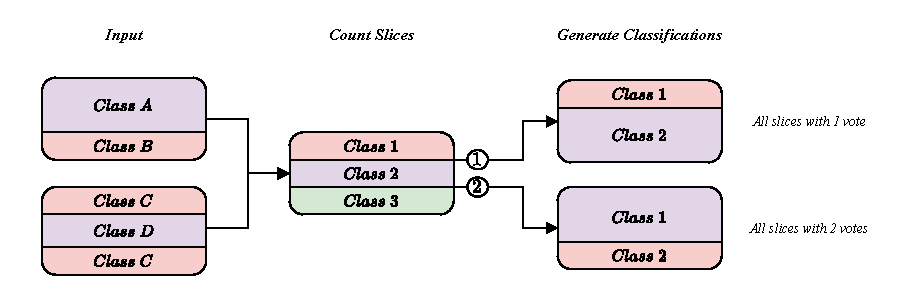
\includegraphics[scale=1.05]{Bilder/DrawIO/strat_ordered_voting_pdf}
					\caption{text}
					\label{fig:tree:classifiers:ovoting}
				\end{figure}
			
				In order to derive a simple and efficient algorithmic approach to this problem, we can make an additional assumptions not based on the model itself, but on its representation in common input formats like \lstinline|.lp| and \lstinline|.mps| files.
				A lot of models are generated via. scripts and written to such files for portability and interoperability with other solvers.
				One exploitable property which can be observed in a lot of models is, that groups constraints are usually \textit{added in bulk}.
				This results in consecutive blocks of constraints which are semantically related, which is illustrated in the \enquote{Input} column of Figure \ref{fig:tree:classifiers:ovoting}.
				If a class of constraints is split into two non-consecutive groups like the second partition from Figure \ref{fig:tree:classifiers:ovoting}, then we can deduce that they are meant to be two different groups.
			
			\subsubsection{Voting (unordered)}
			\label{chap:tree:classifiers:cooccurence}
			
				If the read model does \textit{not} have the property of properly ordered constraint blocks, a more involved algorithmic approach can be used.
				Here, the general problem can be reduced to group constraints with each other which are \textit{often} assigned to the same class.
					
				\clearpage
		
%	\section{Tree Refinement}
%	% 4 Seiten
%	
%		\begin{figure}[ht!]
%			\centering
%			\includesvg{Bilder/Hierarchy/hierarchy_binpack_NOP}
%			\caption{Test}
%			\label{fig:tree:binpackNOP}
%		\end{figure}
		
	\section{Strategies}
	\label{chap:tree:strategies}
	
		Strategies are \textit{the} central building block of the algorithm and are responsible for refining sets of constraints or variables.
		Let $U$ be a the total set of constraints or variables.
		Each strategy gets a single set $S \subseteq U$ as input and produces a partition $\pi_S \in \Pi(S)$ of that set as output.
		Each set $A_i \in \pi_S$ corresponds to one child node.
		Conceptually, each strategy can be seen as a materialization of a specific splitter function as defined in Section \ref{chap:prelims:partitionref}.
		In the following, we differentiate between re-callable and non re-callable strategies. The former type may be called more than once in any given sub-tree, as the result may depend on the set that is being refined.
		
		\clearpage
	
		\subsection{Slice (Partition)}
		
			\begin{figure}[ht!]
				\centering
				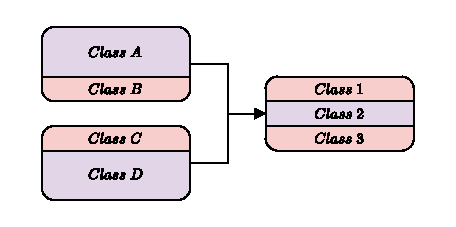
\includegraphics[scale=1.2]{Bilder/DrawIO/strat_slicing_pdf}
				\caption{A simplified illustration assuming that constraint in both partitions can be rearranged into continuous blocks, thus \enquote{slicing} the partitions into different-sized chunks. The output partition inherits all these slices.}
				\label{fig:tree:strat:slice}
			\end{figure}
		
			Slicing strategies are the most simple type of strategy.
			Given two partition $\pi, \pi' \in \Pi(U)$, we define the \textit{combined partition} $\pi \sqcap \pi'$ as follows:
			%
			\begin{equation}
				\label{eq:tree:strat:slice:overlay}
				\pi \sqcap \pi' = \{ A_i \cap B_j \mid A_i \in \pi, B_j \in \pi' \} \setminus \emptyset
			\end{equation}
			%
			This concept is illustrated in Figure \ref{fig:tree:strat:slice}.
			Because strategies only refine single sets and not whole partitions, Equation \ref{eq:tree:strat:slice:overlay} always degenerates to $\pi_{slice} \sqcap \{ S, U \setminus S \}$ for some partition $\pi_{slice} \in \Pi(U)$ and a set $S$ we want to refine.
			The result is then restricted to elements of $S$, which yields a partition of $S$.
			More formally, this strategy can be expressed as Function \ref{eq:tree:strat:slice:function} and computed efficiently using Algorithm \ref{algo:tree:strat:slice}.
			%
			\begin{equation}
			\label{eq:tree:strat:slice:function}
				f(\pi_{splitter}, S) = \left\{ A_i \cap S \mid A_i \in \pi_{splitter} \right\} \setminus \emptyset
			\end{equation}
			%
			Note that the operator $\sqcap$ is trivially associative, i.e., $(\pi \sqcap \pi') \sqcap \pi'' = \pi \sqcap (\pi' \sqcap \pi'')$:
			%
			\begin{alignat*}{4}
				X \in (\pi \sqcap \pi') \sqcap \pi'' &\iff \exists Z \in (\pi \sqcap \pi'), C \in \pi'' && : \; && X && ={} Z \cap C \\
				&\iff \exists A \in \pi, B \in \pi', C \in \pi''&& : \; && X && ={} (A \cap B) \cap C \\
				&\iff \exists A \in \pi, B \in \pi', C \in \pi''&& : \; && X && ={} A \cap (B \cap C) \\
				&\iff  X \in \pi \sqcap (\pi' \sqcap \pi'')
			\end{alignat*}
			
			In conjunction with commutativity, this fact can be used to e.g. eliminate part of the search space by pruning duplicated nodes in the tree and only expanding one instance of any given sub-tree.
		
			\begin{algorithm}[ht!]
				\centering
				\begin{algorithmic}
					\Require Partition $\pi = \{ A_1, A_2, \ldots, A_k \}$, set $S \subseteq U$, function $f_C: U \mapsto \mathbb{N}$ for $C = \{ C_1, C_2, \ldots \} \in \Pi(U)$ mapping $u \in U$ to $C_i$ iff $u \in C_i$
					\Ensure Partition of $S$ according to Function \ref{eq:tree:strat:slice:function}.
					\Statex
					%
					\Function{strategySlice}{$\pi, S$}
						\State $\pi_{out} \gets$ list of $k$ empty sets $B_1, B_2, \ldots, B_k$
						\For{$s \in S$}
							\State $i \gets f_S(s)$
							\State $B_i \gets B_i \cup \{ s \}$
						\EndFor
						\State Remove empty sets from $\pi_{out}$
						\State \Return $\pi_{out}$
					\EndFunction
				\end{algorithmic}
				\caption{If a lookup table represented by function $f$ is available, then Function \ref{eq:tree:strat:slice:function} can be implemented in O($|S|$).}
				\label{algo:tree:strat:slice}
			\end{algorithm}
			
			\FloatBarrier
			\clearpage
		
		\subsection{Slice (Covering)}
		
			Before we explain the \textit{covering} version of the previous strategy, Function \ref{eq:tree:strat:slice:function} can be seen as an instantiation f
		
			This strategy is functionally equivalent to the refinement method \enquote{fast} from \cite{salvagninDetectingSemanticGroups2016}.
			The name most likely stems from an algorithm informally described a fast algorithm based on bucket sort to implement such a partition refinement algorithm.
			
			\clearpage
		
		\subsection{Recursive}

			The \textit{recursive} strategy is the the only strategy which utilizes the full blown partition refinement framework.
			
			\clearpage
			
	
	\section{Scoring}
	% 1 Seite
	
		Up until this point we have only described how the algorithm refines sets based on different strategies, despite the goal being a list of promising partitions.
		Before we describe how to select such partitions, we have to define how we actually \textit{get} a list of partitions from the refinement tree.
		\todo{WIP}
	
		\subsection{Constraint Names}
		\label{chap:tree:scoring:names}
		
			One important piece of information that usually reflects the modelers \textit{intent} when it comes to the semantic difference are the names of the constraints or variables, in the following abbreviated with just \enquote{names}.
			As discusses in Section \ref{chap:gcg:classifiers:name}, names usually consist of multiple parts, with one part containing all the information related to \textit{semantics}.
			Extracting this part of the name can be done heuristically using Algorithm \ref{algo:tree:scoring:nameheur}.
			The heuristic consist of four major steps:
			\begin{enumerate}
				\item Remove \textit{modifies} which are usually enclosed in either brackets or some other special character combination which consists of an \textit{opening} and \textit{closing} character.
				\item \enquote{Normalize} the string by replacing any non-alpha-numeric separators such as spaces, tabs, $\ldots$ with a single character $c$ such as \enquote{\_}.
				\item Split the string according to $c$ and try to detect the part with the relevant semantics. 
				\item \textit{(Optional)} Remove any left-over non-alpha characters such as numbers.
			\end{enumerate}
			
			Step 4 is explicitly marked as optional, because sometimes numbers are integral part of the name, sometimes they are not.
			Both of these cases can actually be observed in the same model \footnote{StrIPlib UUID: d48c9568-e0ea-4c77-9a3b-b7f4dc530d5f}.
			For this model in particular, the constraints \enquote{cut1} to \enquote{cut4} are of interest.
			The constraints with the prefix \enquote{cut1} and \enquote{cut2} are structurally identical, i.e, the they all share the same number of non-zeros and the same type of variables, while \enquote{cut3} and \enquote{cut4} do not.
			Here, \enquote{cut1} and \enquote{cut2} would have to belong to the same group, while \enquote{cut3} and \enquote{cut4} belong in a group their own.
			With the heuristic as is, this case is not detected with or without step 4 because additional information about the actual structure of constraint is required.
			
			Note that the Algorithm makes some implicit key assumptions, such as:
			\begin{itemize}
				\item That the name actually carriers any semantically relevant information at all.
				\item The names adhere to a \enquote{common} format, i.e., the modifier comes \textit{after} the part semantics part.
			\end{itemize}
			
			These assumptions proved reasonable for almost all models observed in practice which had proper names available. Still, there cases where this approach fails \todo{Give MIPLIB examples}.
		
			\begin{algorithm}[ht!]
				\centering
				\begin{algorithmic}
					\Require Name of a constraint
					\Ensure Relevant semantics of the constraint name if the name adheres 
					\Statex
					%
					\Function{extractSemanticPart}{$name$}
						\State ${name}_{new} \gets name$
						\State ${name}_{old} \gets name$
						\Repeat
							\State ${name}_{old} \gets name$
							\State $start \gets$ Position of opening character e.g. $\lbrack$, \{, (, $\ldots$
							\State $end \gets$ Position of corresponding closing character e.g. $\rbrack$, \}, ), $\ldots$
						\Until{${name}_{new} = {name}_{old}$}
					\EndFunction
				\end{algorithmic}
				\caption{}
				\label{algo:tree:scoring:nameheur}
			\end{algorithm}
			\todo{WIP}
			
			\clearpage
			

		\subsection{Ground Truth based}
		% 1 Seite
		
			As discusses in the previous Sections, the algorithm starts with a set in which all constraints or variables are in the same cell.
			In order to \textit{guide} the search towards a plausible semantic partitioning, the existence of a ground-truth partition which approximates the desired partition reasonably well can be used to terminate the search or select promising partitions after the search-space has been explored.
			Terminating the search can, in practice, be very useful, because preventing the algorithm from expanding a node not only prevents unnecessary work being done for this particular node, but also prevents the generation of the entire sub-tree below; reducing the number of potential candidate partitions and overall runtime and space requirements of the algorithm.
			
			Potential sources for a suitable ground-truth partitions include
			\begin{itemize}
				\item Constraint names using the heuristic from Section \ref{chap:tree:scoring:names}. 
				\item Variable information, i.e., given a ground-truth of semantic groupings of variables, one could obtain a corresponding ground-truth partition for constraints by assigning two constraints to different groups iff they contain different kinds of variables according to the ground-truth.
			\end{itemize}
			
			Without the availability of a reasonably ground-truth, it is currently unclear how to know when to terminate the search and more importantly, what structured the desired target partitions should have.
			Here, the term \enquote{structure} refers to all relevant properties of the target partition, including but not limited to, the number and size of the cells.
			
			Assuming a reasonable ground-truth has been obtained, a partition-comparing score such as the Rand-Index already discussed in Section \ref{chap:prelims:rand} can be used a number of promising candidates.
			Furthermore, the refinement can be terminates for sets which are already \textit{homogeneous} according to the ground-truth partition.
			The idea being is that by refining the set further we do not gain any new information.
			
			\clearpage
	
		\subsection{Connected Block Score}
		% 1 Seite
	
			Connected

			\clearpage